%!TEX option = --enable-write18

\documentclass[8pt, xcolor={svgnames, x11names}]{beamer}

 \definecolor{saitPurple}{RGB}{112,40,119}
 \definecolor{statsMaroon}{rgb}{0.55, 0, 0}
 \definecolor{saitMaroon}{rgb}{0.55, 0, 0}
 \definecolor{saitRed}{RGB}{224,38,37}
 \definecolor{saitBlue}{rgb}{0, 0.59, 0.85}
 \definecolor{statsDeepBlue}{RGB}{0, 99, 167}
 \definecolor{saitDeepBlue}{RGB}{0, 99, 167}
 \definecolor{LightGrey}{RGB}{200,200,200}
%  \definecolor{boxBG}{RGB}{236, 227, 227}
%  \definecolor{boxBG}{RGB}{242, 233, 223}
\usepackage{xcolor}
\usepackage{cancel}
\usepackage{bm}
\usepackage{graphicx}
\usepackage{hyperref}
\usepackage{adjustbox}
\hypersetup{colorlinks, allcolors=.,urlcolor=structure}
\usepackage{booktabs}  % for top and bottom spacing in table cells, \addlinespace
\usepackage[x11names, svgnames]{xcolor} % for colors in handouts, auto loaded in Beamer?
\usepackage{tikz}
\usetikzlibrary{arrows.meta, math, calc, shadows,bending}
\usetikzlibrary{decorations.markings, decorations.fractals, decorations.text} % for chain, etc.
\usetikzlibrary{intersections}
\usepackage{pgfmath}
\usepackage{ifthen}
\usepgfmodule{oo}
\usetikzlibrary{shadings}
% \usetikzlibrary{decorations.shapes}
\usepackage[many]{tcolorbox}
\tcbuselibrary{skins} % for image boxes
\usepackage[absolute,overlay,showboxes]{textpos}
% \usepackage{textpos}
% \textblockorigin{0.0cm}{0.0cm}  %start all at upper left corner
\TPshowboxesfalse

\newcommand\lb{\linebreak}
\newcommand\Ra{\Rightarrow}
\newcommand\cd{\!\cdot\!}
\newcommand\x{\!\times\!}
\newcommand\pars{\par\smallskip}
\newcommand\parm{\par\medskip}
\newcommand\parb{\par\bigskip}
\renewcommand{\deg}{^\circ}

% counter for resuming enumerated list numbers
\newcounter{resumeenumi}
\newcommand{\suspend}{\setcounter{resumeenumi}{\theenumi}}
\newcommand{\resume}{\setcounter{enumi}{\theresumeenumi}}



% https://tex.stackexchange.com/questions/33703/extract-x-y-coordinate-of-an-arbitrary-point-in-tikz
\makeatletter
\providecommand{\gettikzxy}[3]{%
	\tikz@scan@one@point\pgfutil@firstofone#1\relax
	\edef#2{\the\pgf@x}%
	\edef#3{\the\pgf@y}%
}
\makeatother

\makeatletter
\newcommand{\verbatimfont}[1]{\def\verbatim@font{#1}}%
\makeatother

%%%%%%%%%%%%%%%%%%%%%%%%%%%%%%%%%%%%%%%%%%%%%%%%%%%%%%%%%%%%%%%%%%%%%%%%%%%%%%%%


% \newcommand{\tb}[4][0.8]{
% 	\begin{textblock*}{#1}(#2, #3)
% 		\raggedright
% 		#4
% 	\end{textblock*}
% }

% \def\tb

\newtcolorbox{statsbox}[2][] { 
  colback=white,
  colbacktitle=structure,
  colframe=structure,
  coltitle=white,  
  top=0.25cm,
	bottom=0.125cm,
	left=0mm,
	right=0mm,
  % fonttitle=\itshape\rmfamily,
  halign=flush left, 
  enhanced,
  drop fuzzy shadow,
  attach boxed title to top left={xshift=3.5mm, yshift=-2mm},
  title={#2}, #1}
\newtcolorbox{redbox}{colback=white, colframe=structure, enhanced, drop fuzzy shadow}
\newtcolorbox{titledbox}[1]{colback=white,colframe=structure,title={#1}}
\newtcbox{\tcb}[1][]{colback=white,boxsep=0pt,top=0.5cm,bottom=0.5cm,left=0.5cm,
		right=0.5cm, colframe=structure,  enhanced, drop fuzzy shadow, #1}
\newtcbox{\tcbfig}[1][1]{colback=white,boxsep=0pt,top=0.5cm,bottom=0.5cm,left=0.5cm,
		right=0.5cm, colframe=structure,  enhanced, drop fuzzy shadow, #1}
% tcb title
\newtcbox{\tcbt}[2][]{colback=white,boxsep=0pt,top=5pt,bottom=5pt,left=5pt,
		right=5pt, colframe=structure, enhanced, drop fuzzy shadow,  title={#2}, #1}
% tcb left title
\newtcbox{\tcbtl}[2][]{ colback=white,
  colbacktitle=structure,
  colframe=structure,
  coltitle=white,  
  top=0.25cm,
	bottom=0.125cm,
	left=0mm,
	right=0mm,
  % fonttitle=\bfseries,
  halign=flush left, 
  enhanced,
  drop fuzzy shadow,
  attach boxed title to top left={xshift=3.5mm, yshift=-2mm}, 
	title={#2}, #1}

\newtcbtheorem{myexam}{Example}%
{
	enhanced,
	colback=white,
	colframe=structure,
	% fonttitle=\bfseries,
	fonttitle=\itshape\rmfamily,
	drop fuzzy shadow,
	%description font=\mdseries\itshape,
	attach boxed title to top left={yshift=-2mm, xshift=5mm},
	colbacktitle=structure
	}{exam}% then \pageref{exer:theoexample} references the theo

% \newcommand{\myexample}[2][red]{
% 	% \tcb\tcbset{theostyle/.style={colframe=red,colbacktitle=yellow}}
% 	\begin{myexam}{}{}
% 		#2
% 	\end{myexam}
% 	% \tcbset{colframe=structure,colbacktitle=structure}
% }

\newtcbtheorem{myexer}{Exercise}%
{
	enhanced,
	colback=white,
	colframe=structure,
	% fonttitle=\bfseries,
	drop fuzzy shadow,
	fonttitle=\itshape\rmfamily,
	% description font=\mdseries\itshape,
	attach boxed title to top left={yshift=-2mm, xshift=5mm},
	colbacktitle=structure
	}{exer}



\newcommand{\mini}[2][0.8]{
	\begin{minipage}[c]{#1\columnwidth}
		\raggedright
		#2
	\end{minipage}
}
\newcommand{\minit}[2][0.8]{
	\begin{minipage}[t]{#1\columnwidth}
		% \raggedright
		#2
	\end{minipage}
}

% centered minipage with text \raggedright
%\cmini[width]{content}
\newcommand{\cmini}[2][0.8]{
	\begin{center}
		\begin{minipage}{#1\columnwidth}
			\raggedright
			#2
		\end{minipage}
	\end{center}
}

\newcommand{\fig}[2][1]{% scaled graphic
	\includegraphics[scale=#1]{#2}
}

% centred framed box black border
%\cbox[width]{content}
\newcommand{\cbox}[2][1]{% framed centered color box
	\setlength\fboxsep{5mm}
	\setlength\fboxrule{.2 mm}
	\begin{center}
		\fcolorbox{black}{white}{
			\vspace{-0.5cm}
			\begin{minipage}{#1\columnwidth}
				\raggedright
				#2
			\end{minipage}
		}
	\end{center}
	\setlength\fboxsep{0cm}
}

\newcommand{\ccbox}[4][1]{% framed centered color box
	\setlength\fboxsep{5mm}
	\setlength\fboxrule{.2 mm}
	\begin{center}
		\fcolorbox{#2}{#3}{
			% \vspace{-0.5cm}
			\begin{minipage}{#1\columnwidth}
				\vspace{-0.25cm}
				\raggedright				
				#4
				\vspace{-0.325cm}
			\end{minipage}
		}
	\end{center}
	\setlength\fboxsep{0cm}
}

\newcommand{\cfig}[2][1]{% centred, scaled graphic
	\begin{center}
		% \fcolorbox{structure}{white}{
		\tcbincludegraphics{
			\includegraphics[scale=#1]{#2}
		}
	\end{center}
}

% figure with tight border for photos
% \cfigb[saitMaroon]{borderwidth with unit}{scale}{image}
\newcommand{\stcsfig}[2][1]{
	% \usepackage{adjustbox}
	% \setlength{\fboxrule}{1pt}
	\begin{center}
		\tcbincludegraphics[width=#1\textwidth, boxrule=2pt, top=-3pt, right=-3pt, left=-3pt, bottom=-3pt,colframe=structure, sharp corners, enhanced, drop fuzzy shadow]{#2}
	\end{center}
}






% %\Member{startpt}{endpt}{outer fill color}{inner fill color}{stroke}{height}{radius}{linewidth}
\providecommand{\Member}[8]{
  % name the points
  \coordinate(start) at (#1);
  \coordinate(end) at (#2);
  \edef\ofill{#3}%
  \edef\ifill{#4}%
  \edef\stroke{#5}%
  \edef\height{#6} % cm
  \edef\radius{#7} % cm
  \edef\linewidth{#8} % mm

  \coordinate(delta) at ($ (end)-(start) $);
  \gettikzxy{(delta)}{\dx}{\dy}
  \gettikzxy{(start)}{\sx}{\sy}
  \pgfmathparse{veclen(\dx, \dy)} \let\length\pgfmathresult

  \pgfmathparse{\dx==0}%
  % \ifnum low-level TeX for integers
  \ifnum\pgfmathresult=1 % \dx == 0
    \pgfmathsetmacro{\rot}{\dy > 0 ? 90 : -90}
  \else
    \pgfmathsetmacro{\rot}{\dx > 0 ? atan(\dy / \dx) : 180 + atan(\dy / \dx)}
  \fi

  
   
  \shadedraw[transform canvas = { rotate around = {\rot:(\sx,\sy)}}, line width = \linewidth, rounded corners = \radius mm, top color = \ofill, bottom color = \ofill, middle color = \ifill, draw = \stroke] ($ (start)+(-0.5*\height, 0.5*\height) $) -- ++(\height cm +\length pt, 0 ) -- ++(0, -\height) -- ++ (-\height cm -\length pt, 0) -- cycle;


  \shadedraw[ball color = \ofill!50!\ifill, draw = \stroke] (start) circle (\height/8);
  \shadedraw[ball color = \ofill!50!\ifill, draw = \stroke] (end) circle (\height/8);
  %  \pgfresetboundingbox

  
  


}

%\Member{startpt}{endpt}{outer fill color}{inner fill color}{stroke}{height}{radius}{linewidth}
\providecommand{\Meme}[8]{
  \coordinate(start) at (#1);
  \coordinate(end) at (#2);
  \edef\ofill{#3}%
  \edef\ifill{#4}%
  \edef\stroke{#5}%
  \edef\height{#6} % cm
  \edef\radius{#7} % cm, should be half \height or less
  \edef\linewidth{#8} % mm

  


  \coordinate(delta) at ($ (end)-(start) $);
  \gettikzxy{(delta)}{\dx}{\dy}
  \gettikzxy{(start)}{\sx}{\sy}
  \gettikzxy{(end)}{\ex}{\ey}
  \pgfmathparse{veclen(\dx, \dy)} \let\length\pgfmathresult
  \pgfmathparse{\height*28.435} \let\heightpt\pgfmathresult
  \pgfmathparse{\heightpt/\length} \let\ratio\pgfmathresult
  \pgfmathparse{1/\ratio} \let\inverse\pgfmathresult
  

  \pgfmathparse{\dx==0}%
  % \ifnum low-level TeX for integers
  \ifnum\pgfmathresult=1 % \dx == 0
    \pgfmathsetmacro{\rot}{\dy > 0 ? 90 : -90}
  \else
    \pgfmathsetmacro{\rot}{\dx > 0 ? atan(\dy / \dx) : 180 + atan(\dy / \dx)}
  \fi

  \pgfmathparse{round(mod(abs(\rot),90))} \let\tmp\pgfmathresult
  \pgfmathsetmacro{\rotmod}{\tmp>45?90-\tmp:\tmp}
  \pgfmathparse{(0.007*\rotmod-0.315)/45+1.017} \let\rotfudge\pgfmathresult

  % \pgfmathparse{mod(abs(\rot),90)} \let\moded\pgfmathresult
  % \ifthenelse{\moded>45}{
  %   \pgfmathparse{90-\moded} \let\rotmod\pgfmathresult    
  % }{
  %   \pgfmathparse{div(\moded,1)} \let\rotmod\pgfmathresult   
  % }


  
  \pgfmathparse{1+3.62/(1+(\inverse/0.714)^1.69)} \let\fudge\pgfmathresult
  \pgfmathparse{50*(1-\ratio)*\fudge*\rotfudge} \let\colorstop\pgfmathresult
  \pgfmathparse{(100-\colorstop)} \let\colorstoptwo\pgfmathresult

  \pgfdeclareverticalshading{myshade}{100bp}{%
					color(0bp)=(\ofill);
					% color(\colorstop bp)=(\ofill);
					color(\colorstop bp)=(\ofill);
					color(50 bp)=(\ifill);
					color(\colorstoptwo bp)=(\ofill);
					color(100bp)=(\ofill)}

  % \tikzset{shading=myshade}

  \begin{scope}[rotate around = {\rot:(start)}, rounded corners = \radius cm, shading angle=\rot]
    \begin{scope} 
      \path[clip]($ (start)+(-0.5*\height, 0.5*\height cm) $) rectangle +(\length pt+\height cm, -\height);
      \shade[shading=myshade] ($ (start)+(-0.5*\height, 0.5*\length pt) $) rectangle +(\length pt+\height cm, -\length pt);
    \end{scope}
  \draw[line width=\linewidth, \stroke] ($ (start)+(-0.5*\height, 0.5*\height cm) $) rectangle +(\length pt+\height cm, -\height);

  % \shadedraw[top color=\ofill, bottom color=\ofill, middle color=\ifill, rotate around = {\rot:(start)}, draw=\stroke, rounded corners = \radius cm, , shading angle=\rot] ($ (start)+(-0.5*\height cm, 0.5*\length pt) $) rectangle +(\length pt+\height cm, -\length pt);
  \end{scope}

  % \pgfresetboundingbox


  % \node[orange] at (0,-1) {rot: \rot};  
  % \node[orange] at (0,-1.5) {rotmod: \rotmod};  
  % \node[orange] at (0,-2) {rotfudge: \rotfudge};  
  % \node[orange] at (-2,-1) {stop2: \colorstoptwo};  
  % \node[orange] at (-2,-1.5) {l/h: \inverse};  
  % \node[orange] at (-2,-2) {fudge: \fudge};  

 
  
  \shade[ball color=\ofill] (start) circle (\height/4);
  \shade[ball color=\ofill] (end) circle (\height/4);

  % \draw(current bounding box.south west) rectangle (current bounding box.north east);


}

\newcommand{\PC}[6][0]{%
  \edef\lrotate{#1}%
  \edef\lpin{#2}%
  \edef\lfill{#3}%
  \edef\ldraw{#4}%
  \edef\lscale{#5}%
  \edef\lwidth{#6}%
  \edef\h{1}%
  \edef\r{0.3}%
  \begin{scope}[scale=\lscale, rotate=\lrotate]
	\filldraw[draw=\ldraw, fill=\lfill, line width=\lwidth mm] ($ (\lpin) + (0.201*\h+1.0353*\r ,-0.75*\h) $) -- ++(105: 0.77646*\h+0.26795*\r) arc (15:165:\r) -- ++(-105:0.77646*\h+0.26795*\r) -- cycle;

	\shadedraw[ball color=\lfill, draw=\ldraw, line width = \lwidth mm] (\lpin) circle (1.5mm);

	\filldraw[rounded corners=\lscale pt, draw=\ldraw, fill=\lfill, line width=\lwidth mm] ($ (\lpin) - (1,1) $) rectangle +(2,0.25);
  \end{scope}%
}





%\Rocker[rotate=0]{coordinate}{draw}{fill}{scale}{line width}
\newcommand{\Rocker}[6][0]{%
	\edef\rotate{#1}%
	\edef\pin{#2}%
	\edef\lfill{#3}%
	\edef\ldraw{#4}%
	\edef\lScale{#5}%
	\edef\lwidth{#6}%
	\edef\h{1}%
	\edef\r{0.3}%

	\begin{scope}[scale=\lScale, rotate=\rotate]

		\filldraw[draw=\ldraw, fill=\lfill, line width = \lwidth mm] ($(\pin) + (0,-\h)$)arc(-90:-57.54:\h) -- ++(105:0.95394)arc(15:165:\r) -- ++(-105:0.95394)arc(-122.458:-90:\h);

		\shadedraw[ball color=\lfill, \ldraw, line width = \lwidth pt] (\pin) circle (1.5mm);
	\end{scope}
}

% !TEX root = ../Beamer/06EquilibriumOfRigidBodies/06ERB.tex

%\Roller[rotate=0]{coordinate}{draw}{fill}{scale}{line width}
\newcommand{\Roller}[6][0]{%
	\edef\rotate{#1}
	\edef\pin{#2}
	\edef\lfill{#3}
	\edef\ldraw{#4}
	\edef\lscale{#5}
	\edef\lwidth{#6}
	\edef\h{1}
	\edef\r{0.3}
	\edef\rr{0.15}
	\begin{scope}[scale=\lscale, rotate=\rotate, myshade/.style={outer color = \lfill!70!\ldraw, inner color=\lfill!25!white, draw=\ldraw!90!black, line width=\lwidth mm}]
		
		\shadedraw[myshade] ($(\pin) + (0,-\h+\rr)$) circle (\rr);
		\filldraw[\ldraw!50!black]($(\pin) + (0,-\h+\rr)$) circle (0.5mm);

		\shadedraw[myshade] ($(\pin) + (-0.325,-\h+\rr)$) circle (\rr);
		\filldraw[\ldraw!50!black]($(\pin) + (-0.325,-\h+\rr)$) circle (0.5mm);

		\shadedraw[myshade] ($(\pin) + (0.325,-\h+\rr)$) circle (\rr);
		\filldraw[\ldraw!50!black]($(\pin) + (0.325,-\h+\rr)$) circle (0.5mm);

		\filldraw[rounded corners= \lscale pt, draw=\ldraw, fill=\lfill, line width=\lwidth mm] ($(\pin) + (-0.52494*\h,-.8*\h)$) -- ++(1.05*\h, 0) -- ++(105:0.9059)arc(15:165:\r) -- cycle;

		\shadedraw[ball color=\lfill, \ldraw, line width=\lwidth mm] (\pin) circle (1.5mm);
		\filldraw[rounded corners=\lscale pt, draw=\ldraw, fill=\lfill, line width=\lwidth mm] ($ (\pin) - (0.55*\h,0.825*\h) $) rectangle +(1.1*\h,0.2*\h);
	\end{scope}
}

% !TEX root = ../Beamer/06EquilibriumOfRigidBodies/06ERB.tex

%\Rone[rotate=0]{coordinate}{draw}{fill}{scale}{line width}
\newcommand{\Rone}[6][0]{
	\def\rotate{#1};
	\def\pin{#2}
	\def\lfill{#3}
	\def\ldraw{#4}
	\def\lScale{#5}
	\def\lwidth{#6}
	\def\h{1}
	\def\r{0.3}

	\begin{scope}[scale=\lScale, rotate=\rotate, line width=\lwidth mm]

		\shadedraw[ball color=\lfill!35!white] ($ (\pin) + (0,-0.6*\h)$) circle (\h*4 mm);
		\filldraw[draw=\ldraw, fill=\lfill] ($(\pin) + (-0.52494*\h,-.8*\h)$) -- ++(1.05*\h, 0) -- ++(105:0.9059)arc(15:165:\r) -- cycle;
		\shadedraw[ball color=\lfill, draw=\ldraw] (\pin) circle (\lScale mm);
		\shadedraw[ball color=\lfill, draw=\ldraw] ($ (\pin) + (0,-0.6*\h)$) circle (\h*0.5 mm);



	\end{scope}
}


\usepackage{mathtools}
\usefonttheme[onlymath]{serif} 
\usepackage{mathpazo} % for mathpazo font
% \usepackage{gensymb} % for \degree
\usepackage[detect-all]{siunitx}
\usepackage{bm}

\setbeamertemplate{navigation symbols}{} % remove navigation symbols
\setbeamertemplate{headline}{\vspace{0.125cm}}
% \setbeamertemplate{footline}{ \hfill \insertshorttitle\qquad \insertsection \qquad \insertframenumber/\inserttotalframenumber\quad{ }\vspace{0.125cm}}
\setbeamertemplate{footline}{ \hfill \insertshorttitle\qquad \insertsection \qquad\vspace{0.125cm}}
\setbeamertemplate{items}[default]
\setbeamertemplate{blocks}[shadow=true]

\usepackage{tikz}
\usetikzlibrary{arrows.meta, math, calc, shadings}
\usepackage{pgfmath}
\usepackage{cancel}
\usepackage[absolute,overlay]{textpos}
\setlength{\TPHorizModule}{1.0cm}
\setlength{\TPVertModule}{\TPHorizModule}
\textblockorigin{0.0cm}{0.0cm}  %start all at upper left corner
% \textblockcolor{yellow}
\usepackage[many]{tcolorbox}
% \usepgflibrary{shadings}

\colorlet{boxBG}{Ivory3!50}


\usecolortheme[named=statsMaroon]{structure}
\setbeamercolor{title}{bg=statsMaroon, fg=boxBG}
\setbeamercolor{frametitle}{fg=boxBG, bg=statsMaroon}
\setbeamercolor{block title}{bg=statsMaroon, fg=boxBG}
\setbeamercolor{block body}{bg=MistyRose, fg=black}

\setlength{\parskip}{\medskipamount}
\setlength{\parindent}{0pt}

\renewcommand{\ttdefault}{pcr}

\def\scale{1}

% https://tex.stackexchange.com/questions/731957/how-to-supress-missing-character-there-is-no-u003b-in-font-nullfont
\tracinglostchars=1

\hfuzz=110pt % suppress Overfull \hbox warnings, up to specified size
\vfuzz=100pt
%%%%%%%%%%%%%%%%%%%%%%%%%%%%%%%%%%%%%%%%%%%%%%%%%%%%%%%%%%%%%%%%%%%%%%%%%%%%%%%%%%%%%%%%%%%%%%%%%%%%
\title[Method of Sections]{\huge \textcolor{white}{Method of Sections --- Step by Step Examples}}
\subtitle[]{\Large\textcolor{white}{Engineering Statics}}

\date{Last revision on \today}

%%%%%%%%%%%%%%%%%%%%%%%%%%%%%%%%%%%%%%%%%%%%%%%%%%%%%%%%%%%%%%%%%%%%%%%%%%%%%%%%%%%%%%%%%%%%%%%%%%%%
\begin{document}
%%%%%%%%%%%%%%%%%%%%%%%%%%%%%%%%%%%%%%%%%%%%%%%%%%%%%%%%%%%%%%%%%%%%%%%%%%%%%%%%%%%%%%%%%%%%%%%%%%%%
\small
%%%%%%%%%%%%%%%%%%%%%%%%%%%%%%%%%%%%%%%%%%%%%%%%%%%%%%%%%%%%%%%%%%%%%%%%%%%%%%%%%%%%%%%%%%%%%%%%%%%%
\begin{frame}[plain]
    \titlepage
\end{frame}
%%%%%%%%%%%%%%%%%%%%%%%%%%%%%%%%%%%%%%%%%%%%%%%%%%%%%%%%%%%%%%%%%%%%%%%%%%%%%%%%%%%%%%%%%%%%%%%%%%%%
\section{Example 2}
%%%%%%%%%%%%%%%%%%%%%%%%%%%%%%%%%%%%%%%%%%%%%%%%%%%%%%%%%%%%%%%%%%%%%%%%%%%%%%%%%%%%%%%%%%%%%%%%%%%%
% \begin{frame}

%   \begin{textblock*}{0.9\paperwidth}(0.875cm, 0.5cm)
%     \def\scale{0.5}\centering
%     \input{../../pikz/08MoS/08MoSSxS02.tex}
%   \end{textblock*}

%   \only<1>{  
%     \begin{textblock*}{8cm}(2.5cm, 5.5cm)
%       \normalsize
%       \begin{statsbox}[colback=NavajoWhite3!37]{Method of Sections: Example 2}
%         \centering
%         Use the method of sections to determine the forces in members $BC$, $CH$ and $GH$.
%       \end{statsbox}
%     \end{textblock*}
%   }
%   \only<2-8>{  
%     \begin{textblock*}{6cm}(0.5cm, 5cm)      
%       \begin{statsbox}[colback=NavajoWhite3!37, left=-2mm, right=2mm, height=3.625cm]{}
%         \centering
%         \begin{itemize}
%           \item<2-> Section $a\mm a$ is the obvious choice for exposing the forces in members $BC$, $CH$ and $GH$.
%           \item<3-> There is no clear advantage to using one side of the section over the other.  Each side has one load and one reaction to consider. We shall use the right portion of the truss, simply because then we don't have to find $R_A$.
%           \item<4-> Find the reaction at $E$.
%           \item<6-> Now for some angles...
%           \suspend
%         \end{itemize}        
%       \end{statsbox}
%     \end{textblock*}
%   }
%   \only<9-10>{  
%     \begin{textblock*}{6cm}(0.5cm, 5cm)      
%       \begin{statsbox}[colback=NavajoWhite3!37, left=-2mm, right=2mm, height=3.625cm]{}
%         \centering        
%         \begin{itemize}
%           \resume
%           \item<9-> Taking moments about the intersection of the lines of action of two of the required forces allows us to solve for the third unknown without resorting to solving simultaneous equations. Thus, taking moments about $C$ will give direct access to $F_{GH}$.
%           \item <10-> Similarly, moments about $H$ yield $F_{BC}$.
%           \suspend   
%         \end{itemize}             
%       \end{statsbox}
%     \end{textblock*}
%   }
%   \only<11->{  
%     \begin{textblock*}{6cm}(0.5cm, 5cm)      
%       \begin{statsbox}[colback=NavajoWhite3!37, left=-2mm, right=2mm, height=3.625cm, top=1.5mm]{}
%         \centering
%         \begin{itemize}
%           \resume
%           \item<11-> There are a number of options now: \par $\Sigma F_y=0$ involves $5$ terms; \par $\Sigma F_x=0$ involves $3$ terms; \par $\Sigma M_G=0$ involves $3$ terms.\par We could even recognize that the lines of action of $F_{BC}$ and of $F_{GH}$ intersect at a point $2.90\,\textsf{m}$ to the left of $A$ -- moments about this point would involve $3$ terms. \parm
%           Taking moments about $G$ is a good option.
%         \end{itemize}        
%       \end{statsbox}
%     \end{textblock*}
%   }

%   \only<5>{
%     \begin{textblock*}{5.25cm}(7cm, 5.875cm)      
%       \begin{statsbox}[colback=NavajoWhite3!37, top=0mm]{}
%         \begin{align*}
%           \Sigma M_A &= R_E\cd(11.60\,\textsf{m})-(4.00\,\textsf{kN})\cd(2.90\,\textsf{m})\\[0.25em]
%           &\qquad\qquad - (5.50\,\textsf{kN})\cd(5.80\,\textsf{m})=0\\[0.25em]
%           \Ra R_E &= 3.75\,\textsf{kN}
%         \end{align*}     
%       \end{statsbox}
%     \end{textblock*}
%   }
%     \only<7-8 >{
%       \begin{textblock*}{5.25cm}(7cm, 5cm)      
%         \begin{statsbox}[colback=NavajoWhite3!37, top=0mm, height=3.625cm]{}
%           \begin{align*}
%             \uncover<7->{
%               \angle BCH &=\tan^{-1}\left[\frac{2.50\,\textsf{m}}{2.90\,\textsf{m}}\right]\\[0.25em]
%               &= 40.764\deg\\\\
%             }
%             \uncover<8->{
%               \angle CGH &= \tan^{-1}\left[\frac{2.90\,\textsf{m}}{1.25\,\textsf{m}}\right]\\[0.25em]
%               &= 66.682\deg
%             }
%           \end{align*}     
%         \end{statsbox}
%       \end{textblock*}
%     }
%     \only<9-10>{
%       \begin{textblock*}{5.25cm}(7cm, 5cm)      
%         \begin{statsbox}[colback=NavajoWhite3!37, top=0mm, height=3.625cm, left=1mm]{}
%           \begin{align*}
%             \uncover<9->{
%               \Sigma M_C &= (3.75\,\textsf{kN})\cd(5.80\,\textsf{m})\\
%               &\quad-F_{GH}\cd\sin 66.682\deg\cd(3.75\,\textsf{m})=0\\
%               \Ra F_{GH} &= 6.3159\,\textsf{kN}\\[0.75em]
%             }
%             \uncover<10->{
%               \Sigma M_H &= (3.75\,\textsf{kN})\cd (8.70\,\textsf{m}) \\
%               &\qquad +F_{BC}\cd (2.50\,\textsf{m})\\
%               &\qquad\qquad-(5.50\,\textsf{kN})\cd (2.90\,\textsf{m})=0\\
%               \Ra F_{BC} &= -6.6700\,\textsf{kM}
%             }
%           \end{align*}     
%         \end{statsbox}
%       \end{textblock*}
%     }
%     \only<12->{
%       \begin{textblock*}{5.25cm}(7cm, 5cm)      
%         \begin{statsbox}[colback=NavajoWhite3!37, top=0mm, height=3.625cm, left=1mm]{}
%           \begin{align*}
%             \uncover<12->{
%               \Sigma M_G &= (3.75\,\textsf{kN})\cd(5.80\,\textsf{m})\\
%               &\qquad + F_{CH}\cd\cos 40.764\deg (3.75\,\textsf{m})\\  
%               &\qquad\qquad + F_{BC}\cd (3.75\,\textsf{m})\\
%               &= 21.75\cd\mathsf{kN\cd m}+F_{CH}(2.8403\,\textsf{m})\\
%               &\qquad +(-6.6700\,\textsf{kN})\cd (3.75\,\textsf{m})=0\\\\
%               \Ra F_{CH} &=  1.1486\,\textsf{kN}                       
%             }
%             \uncover<13->{
%               % \Sigma M_H &= (3.75\,\textsf{kN})\cd (8.70\,\textsf{m}) \\
%               % &\qquad +F_{BC}\cd (2.50\,\textsf{m})\\             
%             }
%           \end{align*}     
%         \end{statsbox}
%       \end{textblock*}
%     } 
    
%     \only<14->{
% 			\begin{textblock*}{1 cm}(0.1cm,0.1cm)
% 				\def\modalFill{white} 
% 				\tikz{%color
  \fill[fill=\modalFill, opacity=0.875] (0.1,0.3) rectangle (12.7,9.45);
}	
% 			\end{textblock*}
				
% 			\begin{textblock*}{5cm}(6.75cm,4cm)
% 					\begin{statsbox}[colback=NavajoWhite3!37]{The Answers}
% 						\small
% 						\begin{align*}
% 							BC &= 6.67\,\textsf{kN}\quad\textsf{(Compression)}\\[0.25em]
% 							BE &= 1.15\,\textsf{kN}\quad\textsf{(Tension)}\\[0.25em]
% 							EF &= 6.32\,\textsf{kN}\quad\textsf{(Tension)}
% 						\end{align*}
% 						\par
% 					\end{statsbox}
% 				\end{textblock*}
%     }
  
% \end{frame}


%%%%%%%%%%%%%%%%%%%%%%%%%%%%%%%%%%%%%%%%%%%%%%%%%%%%%%%%%%%%%%%%%%%%%%%%%%%%%%%%%%%%%%%%%%%%%%%%%%%%%
\section{Example 3} %%%%%%%%%%%%%%%%%%%%%%%%%%%%%%%%%%%%%%%%%%%%%%%%%%%%%%%%%%%%%%%%%%%%%%%%%%%%%%%%%%%%%%%%%%%%%%%%%%%%
% 

% \begin{frame}{}

%   \only<1>{
%     \begin{textblock*}{0.9\paperwidth}(0.875cm, 0.5cm)
%       \def\scale{0.5}\centering
%       
%%%%%%%%%%%%%%%%%%%%%%% TRUSS %%%%%%%%%%%%%%%%%%%%%%%%%%%%%%%%%%%%%%%%%%%%%%%%%%%%%%%%%%%%%%%%%%%%%
\begin{tikzpicture}[scale=\scale]

	\footnotesize

	\coordinate (A) at (0,-1.5);
	\coordinate (B)	at (-3, 0.5);
	\coordinate (C) at (-6,2.5);
	\coordinate (D) at (-9,4.5);
	\coordinate (E) at (-12,4.5);
	\coordinate (F) at (-9,6.5);
	\coordinate (G) at (-6,6.5);
	\coordinate (H) at (-3,6.5);
	\coordinate (I) at (0,6.5);
	\coordinate (Eleft) at ($(E)+(-2.25,0)$);
	% \coordinate (top) at ($(F)+(0,2)$);

	\gettikzxy{(A)}{\ax}{\ay}
	\gettikzxy{(B)}{\bx}{\by}
	\gettikzxy{(C)}{\cx}{\cy}
	\gettikzxy{(E)}{\eex}{\eey}
	\gettikzxy{(Eleft)}{\elx}{\ely}
	\gettikzxy{(F)}{\fx}{\fy}
	\gettikzxy{(G)}{\gx}{\gy}
	\gettikzxy{(H)}{\hx}{\hy}
	\gettikzxy{(I)}{\ix}{\iy}
	% \gettikzxy{(top)}{\tx}{\ty}

	\Meme{A}{B}{LightBlue4}{LightBlue3}{black}{0.4}{0.2}{0.125}
	\Meme{C}{B}{LightBlue4}{LightBlue3}{black}{0.4}{0.2}{0.125}
	\Meme{C}{D}{LightBlue4}{LightBlue3}{black}{0.4}{0.2}{0.125}
	\Meme{E}{D}{LightBlue4}{LightBlue3}{black}{0.4}{0.2}{0.125}
	\Meme{E}{F}{LightBlue4}{LightBlue3}{black}{0.4}{0.2}{0.125}
	\Meme{G}{F}{LightBlue4}{LightBlue3}{black}{0.4}{0.2}{0.125}
	\Meme{G}{H}{LightBlue4}{LightBlue3}{black}{0.4}{0.2}{0.125}
	\Meme{I}{H}{LightBlue4}{LightBlue3}{black}{0.4}{0.2}{0.125}
	\Meme{D}{G}{LightBlue4}{LightBlue3}{black}{0.4}{0.2}{0.125}
	\Meme{C}{H}{LightBlue4}{LightBlue3}{black}{0.4}{0.2}{0.125}
	\Meme{B}{I}{LightBlue4}{LightBlue3}{black}{0.4}{0.2}{0.125}
	\Meme{B}{H}{LightBlue4}{LightBlue3}{black}{0.4}{0.2}{0.125}
	\Meme{C}{G}{LightBlue4}{LightBlue3}{black}{0.4}{0.2}{0.125}
	\Meme{D}{F}{LightBlue4}{LightBlue3}{black}{0.4}{0.2}{0.125}	

	\draw[thin, gray] ($(E)+(0,0.5)$)--+(0,3.5);
	\draw[thin, gray] ($(A)+(-0.75,0)$)--(\elx+0.125cm, \ay);
	\draw[thin, gray] (\bx-0.75cm, \by)--(\elx+0.125cm, \by);
	\draw[thin, gray] (\cx-0.75cm, \cy)--(\elx+0.125cm, \cy);
	\draw[thin, gray] (\eex-0.5cm, \eey)--(\elx+0.125cm, \eey);
	\draw[thin, gray] (\fx-0.75cm, \fy)--(\elx+0.125cm, \fy);

	\draw[thin, gray] ($(I)+(0,0.5)$)--+(0,1.5);

	\only<1-2>{
		\fill[LightBlue3!50!LightBlue4] ($(I)+(0.75,2.25)$) rectangle ($(A)+(2,-1.5)$);
		\draw[semithick]  ($(I)+(0.75,2.25)$) rectangle ($(A)+(0.75,-1.5)$);
		\PC[90]{A}{LightBlue4}{black}{0.75}{0.125}
		\PC[90]{I}{LightBlue4}{black}{0.75}{0.125}
	}
	\only<3->{
		\begin{scope}[opacity=0]
			\fill[LightBlue3!50!LightBlue4] ($(I)+(0.75,2.25)$) rectangle ($(A)+(2,-1.5)$);
			\draw[semithick]  ($(I)+(0.75,2.25)$) rectangle ($(A)+(0.75,-1.5)$);
			\PC[90]{A}{LightBlue4}{black}{0.75}{0.125}
			\PC[90]{I}{LightBlue4}{black}{0.75}{0.125}
		\end{scope}
	}

	\only<3->{
		\begin{scope}[rotate around = {-7.5:(\bx/2+\cx/2, \by/2+\gy/4+\hy/4)}]
			\fill[white] (\gx+0.75cm, \gy+0.5cm) rectangle (\bx-0.875cm, \by+0.325cm);
		\end{scope}
		\draw[saitRed, very thick, -latex] (I)--+(1.5,0)node[above] {\small $ R_{Ix} $};
		\draw[saitRed, very thick, -latex] (I)--+(0, 2.125)node[right,yshift=-0.25cm,] {\small $ R_{Iy} $};
		\draw[saitRed, very thick, -latex] (A)--+(-33.69:1.75)node[above, yshift=0.125cm] {\small $ R_{A} $};
	}

	\foreach \coord in {A,B,C}{
		\filldraw[ball color = LightBlue4] (\coord) circle (2pt)node[below left] {$ \coord $};
	};
	\foreach \coord in {D,E}{
		\filldraw[ball color = LightBlue4] (\coord) circle (2pt)node[left, yshift=-0.25cm] {$ \coord $};
	};
	\filldraw[ball color = LightBlue4] (F) circle (2pt)node[xshift=-0.125cm, yshift=0.25cm] {$ F $};
	\draw[thin, gray] ($(F)+(0,0.5)$)--+(0,1.5);
	\filldraw[ball color = LightBlue4] (G) circle (2pt)node[xshift=-0.125cm, yshift=0.25cm] {$ G $};
	\draw[thin, gray] ($(G)+(0,0.5)$)--+(0,1.5);
	\filldraw[ball color = LightBlue4] (H) circle (2pt)node[xshift=0.125cm, yshift=0.25cm] {$ H $};
	\draw[thin, gray] ($(H)+(0,0.5)$)--+(0,1.5);
	\filldraw[ball color = LightBlue4] (I) circle (2pt)node[xshift=-0.125cm, yshift=0.25cm] {$ I $};
	



	



	

	\draw[very thick, -latex, statsMaroon] (B)--+(0,-1.25)node[below, black, yshift=0.75mm]{$ 5.0\,\textsf{kN}$ };
	\draw[very thick, -latex, statsMaroon] (C)--+(0,-1.25)node[left, black, yshift=0.75mm]{$ 5.0\,\textsf{kN}$ };
	\draw[very thick, -latex, statsMaroon] (D)--+(0,-1.25)node[below, black, yshift=0.75mm]{$ 5.0\,\textsf{kN}$ };
	\draw[very thick, -latex, statsMaroon] (E)--+(0,-1.25)node[below, black, yshift=0.75mm]{$ 10.0\,\textsf{kN}$ };

	\draw[latex-latex] (\eex, 8)--(\fx,8)node[midway, fill=white] {$ 2.25\,\textsf{m} $};
	\draw[latex-latex] (\fx, 8)--(\gx,8)node[midway, fill=white] {$ 2.25\,\textsf{m} $};
	\draw[latex-latex] (\gx, 8)--(\hx,8)node[midway, fill=white] {$ 2.25\,\textsf{m} $};
	\draw[latex-latex] (\hx, 8)--(\ix,8)node[midway, fill=white] {$ 2.25\,\textsf{m} $};

	\draw[latex-latex] (\elx+0.75cm, \fy)--(\elx+0.75cm, \eey)node[midway, fill=white] {$ 1.50\,\textsf{m} $};
	\draw[latex-latex] (\elx+0.75cm, \eey)--(\elx+0.75cm, \cy)node[midway, fill=white] {$ 1.50\,\textsf{m} $};
	\draw[latex-latex] (\elx+0.75cm, \cy)--(\elx+0.75cm, \by)node[midway, fill=white] {$ 1.50\,\textsf{m} $};
	\draw[latex-latex] (\elx+0.75cm, \by)--(\elx+0.75cm, \ay)node[midway, fill=white] {$ 1.50\,\textsf{m} $};

	\only<2>{
		\begin{scope}[rotate around = {-7.5:(\bx/2+\cx/2, \by/2+\gy/4+\hy/4)}]
			\draw[very thick] (\bx/2+\cx/2, \by+0.325cm)--(\hx/2+\gx/2, \gy+0.75cm);
			\node[above] at (\bx/2+\cx/2+0.25cm, \by+0.25cm) {$a$};
			\node[above] at (\gx/2+\hx/2-0.1275cm, \gy+0.25cm) {$a$};
		\end{scope}
	}

	
\end{tikzpicture}

%     \end{textblock*}
%   }
%   \only<2->{
%     \begin{textblock*}{5cm}(5.125cm, 0.35cm)
%      \def\scale{0.45}\centering
%       
%%%%%%%%%%%%%%%%%%%%%%% TRUSS %%%%%%%%%%%%%%%%%%%%%%%%%%%%%%%%%%%%%%%%%%%%%%%%%%%%%%%%%%%%%%%%%%%%%
\begin{tikzpicture}[scale=\scale]

	\footnotesize

	\coordinate (A) at (0,-1.5);
	\coordinate (B)	at (-3, 0.5);
	\coordinate (C) at (-6,2.5);
	\coordinate (D) at (-9,4.5);
	\coordinate (E) at (-12,4.5);
	\coordinate (F) at (-9,6.5);
	\coordinate (G) at (-6,6.5);
	\coordinate (H) at (-3,6.5);
	\coordinate (I) at (0,6.5);
	\coordinate (Eleft) at ($(E)+(-2.25,0)$);
	% \coordinate (top) at ($(F)+(0,2)$);

	\gettikzxy{(A)}{\ax}{\ay}
	\gettikzxy{(B)}{\bx}{\by}
	\gettikzxy{(C)}{\cx}{\cy}
	\gettikzxy{(E)}{\eex}{\eey}
	\gettikzxy{(Eleft)}{\elx}{\ely}
	\gettikzxy{(F)}{\fx}{\fy}
	\gettikzxy{(G)}{\gx}{\gy}
	\gettikzxy{(H)}{\hx}{\hy}
	\gettikzxy{(I)}{\ix}{\iy}
	% \gettikzxy{(top)}{\tx}{\ty}

	\Meme{A}{B}{LightBlue4}{LightBlue3}{black}{0.4}{0.2}{0.125}
	\Meme{C}{B}{LightBlue4}{LightBlue3}{black}{0.4}{0.2}{0.125}
	\Meme{C}{D}{LightBlue4}{LightBlue3}{black}{0.4}{0.2}{0.125}
	\Meme{E}{D}{LightBlue4}{LightBlue3}{black}{0.4}{0.2}{0.125}
	\Meme{E}{F}{LightBlue4}{LightBlue3}{black}{0.4}{0.2}{0.125}
	\Meme{G}{F}{LightBlue4}{LightBlue3}{black}{0.4}{0.2}{0.125}
	\Meme{G}{H}{LightBlue4}{LightBlue3}{black}{0.4}{0.2}{0.125}
	\Meme{I}{H}{LightBlue4}{LightBlue3}{black}{0.4}{0.2}{0.125}
	\Meme{D}{G}{LightBlue4}{LightBlue3}{black}{0.4}{0.2}{0.125}
	\Meme{C}{H}{LightBlue4}{LightBlue3}{black}{0.4}{0.2}{0.125}
	\Meme{B}{I}{LightBlue4}{LightBlue3}{black}{0.4}{0.2}{0.125}
	\Meme{B}{H}{LightBlue4}{LightBlue3}{black}{0.4}{0.2}{0.125}
	\Meme{C}{G}{LightBlue4}{LightBlue3}{black}{0.4}{0.2}{0.125}
	\Meme{D}{F}{LightBlue4}{LightBlue3}{black}{0.4}{0.2}{0.125}	

	\draw[thin, gray] ($(E)+(0,0.5)$)--+(0,3.5);
	\draw[thin, gray] ($(A)+(-0.75,0)$)--(\elx+0.125cm, \ay);
	\draw[thin, gray] (\bx-0.75cm, \by)--(\elx+0.125cm, \by);
	\draw[thin, gray] (\cx-0.75cm, \cy)--(\elx+0.125cm, \cy);
	\draw[thin, gray] (\eex-0.5cm, \eey)--(\elx+0.125cm, \eey);
	\draw[thin, gray] (\fx-0.75cm, \fy)--(\elx+0.125cm, \fy);

	\draw[thin, gray] ($(I)+(0,0.5)$)--+(0,1.5);

	\only<1-2>{
		\fill[LightBlue3!50!LightBlue4] ($(I)+(0.75,2.25)$) rectangle ($(A)+(2,-1.5)$);
		\draw[semithick]  ($(I)+(0.75,2.25)$) rectangle ($(A)+(0.75,-1.5)$);
		\PC[90]{A}{LightBlue4}{black}{0.75}{0.125}
		\PC[90]{I}{LightBlue4}{black}{0.75}{0.125}
	}
	\only<3->{
		\begin{scope}[opacity=0]
			\fill[LightBlue3!50!LightBlue4] ($(I)+(0.75,2.25)$) rectangle ($(A)+(2,-1.5)$);
			\draw[semithick]  ($(I)+(0.75,2.25)$) rectangle ($(A)+(0.75,-1.5)$);
			\PC[90]{A}{LightBlue4}{black}{0.75}{0.125}
			\PC[90]{I}{LightBlue4}{black}{0.75}{0.125}
		\end{scope}
	}

	\only<3->{
		\begin{scope}[rotate around = {-7.5:(\bx/2+\cx/2, \by/2+\gy/4+\hy/4)}]
			\fill[white] (\gx+0.75cm, \gy+0.5cm) rectangle (\bx-0.875cm, \by+0.325cm);
		\end{scope}
		\draw[saitRed, very thick, -latex] (I)--+(1.5,0)node[above] {\small $ R_{Ix} $};
		\draw[saitRed, very thick, -latex] (I)--+(0, 2.125)node[right,yshift=-0.25cm,] {\small $ R_{Iy} $};
		\draw[saitRed, very thick, -latex] (A)--+(-33.69:1.75)node[above, yshift=0.125cm] {\small $ R_{A} $};
	}

	\foreach \coord in {A,B,C}{
		\filldraw[ball color = LightBlue4] (\coord) circle (2pt)node[below left] {$ \coord $};
	};
	\foreach \coord in {D,E}{
		\filldraw[ball color = LightBlue4] (\coord) circle (2pt)node[left, yshift=-0.25cm] {$ \coord $};
	};
	\filldraw[ball color = LightBlue4] (F) circle (2pt)node[xshift=-0.125cm, yshift=0.25cm] {$ F $};
	\draw[thin, gray] ($(F)+(0,0.5)$)--+(0,1.5);
	\filldraw[ball color = LightBlue4] (G) circle (2pt)node[xshift=-0.125cm, yshift=0.25cm] {$ G $};
	\draw[thin, gray] ($(G)+(0,0.5)$)--+(0,1.5);
	\filldraw[ball color = LightBlue4] (H) circle (2pt)node[xshift=0.125cm, yshift=0.25cm] {$ H $};
	\draw[thin, gray] ($(H)+(0,0.5)$)--+(0,1.5);
	\filldraw[ball color = LightBlue4] (I) circle (2pt)node[xshift=-0.125cm, yshift=0.25cm] {$ I $};
	



	



	

	\draw[very thick, -latex, statsMaroon] (B)--+(0,-1.25)node[below, black, yshift=0.75mm]{$ 5.0\,\textsf{kN}$ };
	\draw[very thick, -latex, statsMaroon] (C)--+(0,-1.25)node[left, black, yshift=0.75mm]{$ 5.0\,\textsf{kN}$ };
	\draw[very thick, -latex, statsMaroon] (D)--+(0,-1.25)node[below, black, yshift=0.75mm]{$ 5.0\,\textsf{kN}$ };
	\draw[very thick, -latex, statsMaroon] (E)--+(0,-1.25)node[below, black, yshift=0.75mm]{$ 10.0\,\textsf{kN}$ };

	\draw[latex-latex] (\eex, 8)--(\fx,8)node[midway, fill=white] {$ 2.25\,\textsf{m} $};
	\draw[latex-latex] (\fx, 8)--(\gx,8)node[midway, fill=white] {$ 2.25\,\textsf{m} $};
	\draw[latex-latex] (\gx, 8)--(\hx,8)node[midway, fill=white] {$ 2.25\,\textsf{m} $};
	\draw[latex-latex] (\hx, 8)--(\ix,8)node[midway, fill=white] {$ 2.25\,\textsf{m} $};

	\draw[latex-latex] (\elx+0.75cm, \fy)--(\elx+0.75cm, \eey)node[midway, fill=white] {$ 1.50\,\textsf{m} $};
	\draw[latex-latex] (\elx+0.75cm, \eey)--(\elx+0.75cm, \cy)node[midway, fill=white] {$ 1.50\,\textsf{m} $};
	\draw[latex-latex] (\elx+0.75cm, \cy)--(\elx+0.75cm, \by)node[midway, fill=white] {$ 1.50\,\textsf{m} $};
	\draw[latex-latex] (\elx+0.75cm, \by)--(\elx+0.75cm, \ay)node[midway, fill=white] {$ 1.50\,\textsf{m} $};

	\only<2>{
		\begin{scope}[rotate around = {-7.5:(\bx/2+\cx/2, \by/2+\gy/4+\hy/4)}]
			\draw[very thick] (\bx/2+\cx/2, \by+0.325cm)--(\hx/2+\gx/2, \gy+0.75cm);
			\node[above] at (\bx/2+\cx/2+0.25cm, \by+0.25cm) {$a$};
			\node[above] at (\gx/2+\hx/2-0.1275cm, \gy+0.25cm) {$a$};
		\end{scope}
	}

	
\end{tikzpicture}

%     \end{textblock*}
%   }

%   \only<1>{  
%     \begin{textblock*}{8cm}(2.5cm, 6.75cm)
%       \normalsize
%       \begin{statsbox}[colback=NavajoWhite3!37]{Method of Sections: Example 3}
%         \centering
%         Use the method of sections to determine the forces in members $BC$, $CH$ and $GH$.
%       \end{statsbox}
%     \end{textblock*}
%   }

%   \only<2-5>{  
%     \begin{textblock*}{6cm}(0.5cm, 5.625cm)      
%       \begin{statsbox}[colback=NavajoWhite3!37, left=-2mm, right=2mm, height=3.25cm]{}
%         \centering
%         \begin{itemize}
%           \item<2-> Draw section $a\mm a$ to expose the forces in members $BC$, $CH$ and $GH$.
%           \item<3-> The right portion of the truss involves solving for the reactions, and then including these reactions in all our calculations. Although the left portion has more applied loads, it is still the more convenient option. 
%           \item<5-> Find the angles we'll need...
%         \end{itemize}        
%       \end{statsbox}
%     \end{textblock*}
%   }

%   \only<5>{
%     \begin{textblock*}{5.25cm}(7cm, 5.625cm)      
%       \begin{statsbox}[colback=NavajoWhite3!37, top=0mm, height=3.25cm]{}
%         \begin{align*}
%           \theta &= \tan^{-1}\left[\frac{1.50\,\textsf{m}}{2.25\,\textsf{m}}\right]=33.690\deg\\\\
%           \phi &= \tan^{-1}\left[\frac{3.00\,\textsf{m}}{2.25\,\textsf{m}}\right]=53.130\deg       
%         \end{align*}     
%       \end{statsbox}
%     \end{textblock*}
%   }

%   \only<6->{  
%     \begin{textblock*}{5cm}(0.5cm, 5.625cm)      
%       \begin{statsbox}[colback=NavajoWhite3!37, left=-2mm, right=2mm, height=3.5cm]{}
%         \centering        
%         \begin{itemize}         
%           \item<6-> Sum moments about $C$ to find $F_{GH}$.
%           \item <7-> In this example, it is probably simplest now to sum both the $x$-components and the $y$-components,
%           \uncover<8->{ and to then solve the resulting system of equations.}          
%         \end{itemize}             
%       \end{statsbox}
%     \end{textblock*}
%   }

%   \only<6>{
%     \begin{textblock*}{6.25cm}(6cm, 5.625cm)      
%       \begin{statsbox}[colback=NavajoWhite3!37, top=0mm, height=3.5cm]{}
%         \begin{align*}
%           \Sigma M_C &= (10.0\,\textsf{kN})\cd (4.50\,\textsf{m})\\[0.25em]
%           &\qquad +(5.0\,\textsf{kN})\cd (2.25\,\textsf{m})\\[0.25em] 
%           &\qquad\qquad - F_{GH}(3.00\,\textsf{m}) = 0 \\\\
%           \Ra F_{GH} &= 18.750\,\textsf{kN}
%         \end{align*}     
%       \end{statsbox}
%     \end{textblock*}
%   }

%   \only<7>{
%     \begin{textblock*}{6.25cm}(6cm, 5.625cm)      
%       \begin{statsbox}[colback=NavajoWhite3!37, top=0mm, height=3.5cm]{}
%         \begin{align*}
%           \Sigma F_x &= F_{GH}+F_{CH}\cd\cos\phi +F_{BC}\cd\cos\theta \\[0.25em]
%           &= 18.750\,\textsf{kN} + F_{CH}\cd 0.60000\,\textsf{kN} + F_{BC}\cd 0.83205\,\textsf{kN}\\[0.25em]
%           &=0\\\\
%           \Sigma F_y &= F_{CH}\cd\sin\phi -F_{BC}\cd\sin\theta-20.0\,\textsf{kN}\\[0.25em]
%           &= F_{CH}\cd 0.80000\,\textsf{kN} - F_{BC}\cd 0.55470\,\textsf{kN}-20.0\,\textsf{kN}\\[0.25em]
%           &=0
%         \end{align*}     
%       \end{statsbox}
%     \end{textblock*}
%   }

%   \only<8->{
%     \begin{textblock*}{6.25cm}(6cm, 5.625cm)      
%       \begin{statsbox}[colback=NavajoWhite3!37, top=0mm, height=3.5cm]{}
%         \begin{align*}
%           0.83205\cd F_{BC}+0.60000\cd F_{CH} &= -18.750\,\textsf{kN} \\[0.25em]
%           0.55470\cd F_{BC}-0.80000\cd F_{CH} &= -20.0\,\textsf{kN}     
%         \end{align*}
%         From the system-solver:
%         \begin{align*}
%           F_{BC} & = -27.042\,\textsf{kN}\\[0.25em]   
%           F_{CH} & = 6.2500\,\textsf{kN}
%         \end{align*}
%       \end{statsbox}
%     \end{textblock*}
%   }

%   \only<9->{
%     \begin{textblock*}{1 cm}(0.1cm,0.1cm)
%       \def\modalFill{white} 
%       \tikz{%color
  \fill[fill=\modalFill, opacity=0.875] (0.1,0.3) rectangle (12.7,9.45);
}	
%     \end{textblock*}
				
%     \begin{textblock*}{5cm}(6.75cm,4cm)
%       \begin{statsbox}[colback=NavajoWhite3!37]{The Answers}
%         \small
%         \begin{align*}
%           BC &= 27.0\,\textsf{kN}\quad\textsf{(Compression)}\\[0.25em]
%           CH &= 6.25\,\textsf{kN}\quad\textsf{(Tension)}\\[0.25em]
%           GH &= 18.8\,\textsf{kN}\quad\textsf{(Tension)}						
%         \end{align*}
%         \par
%       \end{statsbox}
%     \end{textblock*}
%   }
  
% \end{frame}



%%%%%%%%%%%%%%%%%%%%%%%%%%%%%%%%%%%%%%%%%%%%%%%%%%%%%%%%%%%%%%%%%%%%%%%%%%%%%%%%%%%%%%%%%%%%%%%%%%%

%%%%%%%%%%%%%%%%%%%%%%%%%%%%%%%%%%%%%%%%%%%%%%%%%%%%%%%%%%%%%%%%%%%%%%%%%%%%%%%%%%%%%%%%%%%%%%%%%%%%%
\section{Example 4} %%%%%%%%%%%%%%%%%%%%%%%%%%%%%%%%%%%%%%%%%%%%%%%%%%%%%%%%%%%%%%%%%%%%%%%%%%%%%%%%%%%%%%%%%%%%%%%%%%%%



\begin{frame}{}

  \only<1>{
    \begin{textblock*}{12.8cm}(0cm, 0.25cm)
      \def\scale{0.5}\centering
      
%%%%%%%%%%%%%%%%%%%%%%% TRUSS %%%%%%%%%%%%%%%%%%%%%%%%%%%%%%%%%%%%%%%%%%%%%%%%%%%%%%%%%%%%%%%%%%%%%
\begin{tikzpicture}[scale=\scale, line cap = round]

	\footnotesize

	\coordinate (A) at (0,0);
	\coordinate (B)	at (3,2);
	\coordinate (C) at (6,4);
	\coordinate (D) at (9,6);
	\coordinate (E) at (12,4);
	\coordinate (DE) at (10.5,5);
	\coordinate (F) at (15,2);
	\coordinate (G) at (18,0);
	\coordinate (H) at (15,0);
	\coordinate (I) at (12,0);
	\coordinate (J) at (9,0);
	\coordinate (EJ) at (10.5,2);
	\coordinate (EJJ) at ($ (E)!0.65!(J) $);
	\coordinate (CDD) at ($ (D)!0.35!(C) $);
	\coordinate (DJJ) at ($ (D)!0.45!(J) $);
	\coordinate (IJ) at (10.5,0);
	\coordinate (IJJ) at ($ (I)!0.35!(J) $);
	\coordinate (K) at (6,0);
	\coordinate (L) at (3,0);
	

	\gettikzxy{(A)}{\ax}{\ay}
	\gettikzxy{(B)}{\bx}{\by}
	\gettikzxy{(C)}{\cx}{\cy}
	\gettikzxy{(D)}{\ddx}{\ddy}
	\gettikzxy{(E)}{\eex}{\eey}
	\gettikzxy{(DE)}{\dex}{\dey}
	\gettikzxy{(F)}{\fx}{\fy}
	\gettikzxy{(G)}{\gx}{\gy}
	\gettikzxy{(H)}{\hx}{\hy}
	\gettikzxy{(I)}{\ix}{\iy}
	\gettikzxy{(J)}{\jx}{\jy}
	
	\only<1-8>{
		\Meme{C}{B}{NavajoWhite4}{NavajoWhite2}{black}{0.4}{0.2}{0.125}
		\Meme{C}{D}{NavajoWhite4}{NavajoWhite2}{black}{0.4}{0.2}{0.125}
		\Meme{E}{D}{NavajoWhite4}{NavajoWhite2}{black}{0.4}{0.2}{0.125}
		\Meme{K}{J}{NavajoWhite4}{NavajoWhite2}{black}{0.4}{0.2}{0.125}
		\Meme{K}{L}{NavajoWhite4}{NavajoWhite2}{black}{0.4}{0.2}{0.125}
		\Meme{A}{L}{NavajoWhite4}{NavajoWhite2}{black}{0.4}{0.2}{0.125}
		\Meme{A}{B}{NavajoWhite4}{NavajoWhite2}{black}{0.4}{0.2}{0.125}
		\Meme{B}{K}{NavajoWhite4}{NavajoWhite2}{black}{0.4}{0.2}{0.125}
		\Meme{C}{J}{NavajoWhite4}{NavajoWhite2}{black}{0.4}{0.2}{0.125}
		
		\Meme{I}{J}{NavajoWhite4}{NavajoWhite2}{black}{0.4}{0.2}{0.125}
		\Meme{E}{J}{NavajoWhite4}{NavajoWhite2}{black}{0.4}{0.2}{0.125}
		\Meme{D}{J}{NavajoWhite4}{NavajoWhite2}{black}{0.4}{0.2}{0.125}
		\Meme{B}{L}{NavajoWhite4}{NavajoWhite2}{black}{0.4}{0.2}{0.125}
		\Meme{C}{K}{NavajoWhite4}{NavajoWhite2}{black}{0.4}{0.2}{0.125}
	}	
	\only<9->{
		\Meme{C}{B}{Cornsilk3}{white}{gray!50}{0.4}{0.2}{0.125}
		\Meme{C}{D}{Cornsilk3}{white}{gray!50}{0.4}{0.2}{0.125}
		\Meme{DE}{D}{Cornsilk3}{white}{gray!50}{0.4}{0.2}{0.125}		
		\Meme{K}{J}{Cornsilk3}{white}{gray!50}{0.4}{0.2}{0.125}
		\Meme{K}{L}{Cornsilk3}{white}{gray!50}{0.4}{0.2}{0.125}
		\Meme{A}{L}{Cornsilk3}{white}{gray!50}{0.4}{0.2}{0.125}
		\Meme{A}{B}{Cornsilk3}{white}{gray!50}{0.4}{0.2}{0.125}
		\Meme{B}{K}{Cornsilk3}{white}{gray!50}{0.4}{0.2}{0.125}
		\Meme{C}{J}{Cornsilk3}{white}{gray!50}{0.4}{0.2}{0.125}		
		\Meme{IJ}{J}{Cornsilk3}{white}{gray!50}{0.4}{0.2}{0.125}		
		\Meme{EJ}{J}{Cornsilk3}{white}{gray!50}{0.4}{0.2}{0.125}		
		\Meme{D}{J}{Cornsilk3}{white}{gray!50}{0.4}{0.2}{0.125}
		\Meme{B}{L}{Cornsilk3}{white}{gray!50}{0.4}{0.2}{0.125}
		\Meme{C}{K}{Cornsilk3}{white}{gray!50}{0.4}{0.2}{0.125}
		\Meme{IJJ}{I}{NavajoWhite4}{NavajoWhite2}{black}{0.4}{0.2}{0.125}
	}	
	\only<9-10>{
	\Meme{E}{DE}{NavajoWhite4}{NavajoWhite2}{black}{0.4}{0.2}{0.125}	
	\Meme{EJ}{E}{NavajoWhite4}{NavajoWhite2}{black}{0.4}{0.2}{0.125}
	}
	\only<10->{		
		\Meme{D}{CDD}{NavajoWhite4}{NavajoWhite2}{black}{0.4}{0.2}{0.125}
		\Meme{D}{E}{NavajoWhite4}{NavajoWhite2}{black}{0.4}{0.2}{0.125}
		\Meme{D}{DJJ}{NavajoWhite4}{NavajoWhite2}{black}{0.4}{0.2}{0.125}
		\Meme{E}{EJJ}{NavajoWhite4}{NavajoWhite2}{black}{0.4}{0.2}{0.125}
	}
	
	\Meme{E}{F}{NavajoWhite4}{NavajoWhite2}{black}{0.4}{0.2}{0.125}	
	\Meme{G}{H}{NavajoWhite4}{NavajoWhite2}{black}{0.4}{0.2}{0.125}
	\Meme{I}{H}{NavajoWhite4}{NavajoWhite2}{black}{0.4}{0.2}{0.125}	
	\Meme{G}{F}{NavajoWhite4}{NavajoWhite2}{black}{0.4}{0.2}{0.125}	
	\Meme{F}{I}{NavajoWhite4}{NavajoWhite2}{black}{0.4}{0.2}{0.125}	
	\Meme{E}{I}{NavajoWhite4}{NavajoWhite2}{black}{0.4}{0.2}{0.125}
	\Meme{F}{H}{NavajoWhite4}{NavajoWhite2}{black}{0.4}{0.2}{0.125}

	\only<1-8>{
		\fill[DarkSeaGreen4] ($(A)+(-1,-0.75)$) rectangle +(2,-0.5);
		\fill[DarkSeaGreen4] ($(G)+(-1,-0.75)$) rectangle +(2,-0.5);
		\PC{G}{DarkSeaGreen4}{black}{0.75}{0.2}
		\Roller{A}{DarkSeaGreen4}{black}{0.75}{0.2}
		\filldraw[ball color = NavajoWhite4] (A) circle (4pt);
		\filldraw[ball color = NavajoWhite4] (G) circle (4pt);
	}
	

	\draw[thin, gray]($ (A)+(0,-1.5)$)--+(0,-1.75);
	\draw[thin, gray]($ (G)+(0,-1.5)$)--+(0,-1.75);
	\draw[thin, gray]($ (J)+(0,-.5)$)--+(0,-2.75);
	\draw[thin, gray]($ (H)+(0,-.5)$)--+(0,-2.75);
	\draw[thin, gray]($ (L)+(0,-2)$)--+(0,-1.25);
	\draw[thin, gray]($ (K)+(0,-2)$)--+(0,-1.25);
	\draw[thin, gray]($ (I)+(0,-2)$)--+(0,-1.25);
	\draw[thin, gray]($ (A)+(-0.5,0)$)--(-2, \ay);
	\draw[thin, gray]($ (B)+(-0.75,0)$)--(-2, \by);
	\draw[thin, gray]($ (C)+(-0.75,0)$)--(-2, \cy);
	\draw[thin, gray]($ (D)+(-0.75,0)$)--(-2, \ddy);

	\foreach \x in {0,1,2,...,5} {
		\draw[latex-latex] (\x*3, -2.625)--+(3,0)node[midway, fill=white]{$ 4.25\,\textsf{m} $};
	}
	\draw[latex-latex] (\ax-1.125cm, \ay)--(\ax-1.125cm, \by)node[midway, fill=white, inner sep = 0.5mm]{$ 2.75\,\textsf{m} $};
	\draw[latex-latex] (\ax-1.125cm, \by)--(\ax-1.125cm, \cy)node[midway, fill=white]{$ 2.75\,\textsf{m} $};
	\draw[latex-latex] (\ax-1.125cm, \cy)--(\ax-1.125cm, \ddy)node[midway, fill=white]{$ 2.75\,\textsf{m} $};

	\only<1-8>{
		\draw[very thick, -latex, statsRed] (L)--+(0,-1.25)node[below,  yshift=0.75mm]{$ 5.00\,\textsf{kN}$ };
		\draw[very thick, -latex, statsRed] (K)--+(0,-1.25)node[below, yshift=0.75mm]{$ 5.00\,\textsf{kN}$ };		
	}
	\draw[very thick, -latex, statsRed] (I)--+(0,-1.25)node[below,  yshift=0.75mm]{$ 10.0\,\textsf{kN}$ };

	\only<2-3>{
		\begin{scope}[rotate around = {25:(\ddx, \ddy/2+\jy/2)}]
			\draw[ultra thick,Green3] (\ddx, \ddy)--(\ddx, \jy-0.75cm);
			\node at (\ddx-0.25cm, \ddy) {$a$};
			\node at (\jx-0.325cm, \jy-0.75cm) {$a$};
		\end{scope}
	}
	\only<3>{
			\draw[ultra thick,Green3] (\ddx/3+2*\eex/3, \ddy-0.75cm)--(\ddx/3+2*\eex/3, \jy-0.5cm);
			\node at (\ddx/3+2*\eex/3+0.25cm, \ddy-0.75cm) {$b$};
			\node at (\ddx/3+2*\eex/3+0.25cm, \jy-0.5cm) {$b$};
	}
	\only<4>{
		\draw[saitRed, -latex, very thick] (A)--+(90:1.325)node[above,inner sep = 0.2mm,yshift=-0.2mm]{\small $R_{A}$};
	}
	\only<5-8>{
		\draw[saitRed, -latex, very thick] (A)--+(90:1.325)node[above,xshift=2mm,inner sep = 0.2mm]{ $10.833\,\textsf{kN}$};
	}
	\only<4-5>{
		\draw[saitRed, -latex, very thick] (G)--+(90:1.5)node[above,yshift=-1mm]{\small $R_{Gy}$};				
	}
	\only<6->{
		\draw[saitRed, -latex, very thick] (G)--+(90:1.5)node[above,yshift=-0.2mm]{$9.1670\,\textsf{kN}$};	
	}
	\only<4-6>{
		\draw[saitRed, -latex, very thick] (G)--+(180:1.75)node[below,yshift=-0.2mm]{\small $R_{Gx}$};
	}
	\only<8>{
		\draw[ultra thick,Green3] (\ddx/2+\eex/2, \ddy-0.25em)--(\ddx/2+\eex/2, \jy-0.75cm);
		\node at (\ddx/2+\eex/2+0.25cm, \ddy-0.125cm) {$b$};
		\node at (\ddx/2+\eex/2+0.25cm, \jy-0.75cm) {$b$};
	}
	\only<9>{
		\fill[ultra thick,white] (\ddx/2+\eex/2-0.5cm, \ddy-0.25em)rectangle(\ddx/2+\eex/2+0.5cm, \jy-0.75cm);
		\draw[thick, -latex] ($(E)+(146.3:0.5)$)--+(146.3:1.5)node[above,xshift=1mm]{$F_{DE}$};
		\draw[thick, -latex] ($(E)+(233:0.5)$)--+(233:2)node[above left,outer sep=-0.5mm]{$F_{EJ}$};
		\draw[thick, -latex] ($(I)+(180.3:0.5)$)--+(180:1.25)node[above,xshift=1mm]{$F_{IJ}$};
	}
	\only<10->{
		\begin{scope}[rotate around = {30:(\ddx-0.5cm, \ddy/2+\jy/2)},xshift=0.5cm]
			\fill[white] (\ddx-1cm, \ddy-0.25cm)rectangle(\ddx, \jy-1.325cm);
		\end{scope}
	}
	\only<10>{
		\begin{scope}[rotate around = {30:(\ddx-0.5cm, \ddy/2+\jy/2)},xshift=0.5cm]
			
			\draw[ultra thick,Green3] (\ddx-0.5cm, \ddy-0.125cm)--(\ddx-0.5cm, \jy-1.25cm);
			\node at (\ddx-0.875cm, \ddy) {$a$};
			\node at (\jx-0.875cm, \jy-1.25cm) {$a$};
		\end{scope}
	}
	\only<11->{
		\draw[latex-latex] ($(D)+(213.7:1.5)$)arc(213.7:270:1.5)node[midway, fill=white,inner sep=0.2mm]{\small $\theta$};
		\draw[latex-latex] ($(E)+(233.1:2.5)$)arc(233.1:270:2.5)node[midway, fill=white,inner sep=0.2mm]{\small $\phi$};
	}
	\only<11->{
		\draw[thick, -latex] ($(D)+(213.7:0.5)$)--+(213.7:2)node[above,yshift=1mm]{$\bm{ F_{CD} }$};
		\draw[thick, -latex] ($(D)+(270:1.25)$)--+(270:1.5)node[below,yshift=1mm]{$\bm{ F_{DJ}} $};
		\draw[thick, -latex] ($(E)+(233.1:1.875)$)--+(233.1:1.625)node[left,yshift=1mm,xshift=1mm]{$\bm{ F_{EJ}} $};
		\draw[thick, -latex] ($(I)+(180:0.325)$)--+(180:1.625)node[above,xshift=1mm,yshift=0.5mm]{$ 14.167\,\textsf{kN} $};
	}
	


	

	






	\foreach \coord in {B,C,...,F}{
		\filldraw[ball color = NavajoWhite4] (\coord) circle (3pt)node[yshift=0.325cm] {$ \coord $};
	};
	\foreach \coord in {H, I, J, K, L}{
		\filldraw[ball color = NavajoWhite4] (\coord) circle (3pt)node[left, yshift=-0.25cm] {$ \coord $};		
	};
	
	\filldraw[ball color = NavajoWhite4] (G) circle (3pt)node[xshift=0.25cm, yshift=0.125cm] {$ G $};
	\filldraw[ball color = NavajoWhite4] (A) circle (3pt)node[xshift=-0.25cm, yshift=0.125cm] {$ A $};

	\path(-2.5,-3.5) rectangle (19.5, 7.25);
\end{tikzpicture}

    \end{textblock*}
  }

  \only<2->{
    \begin{textblock*}{12.8cm}(0cm, 0.25cm)
     \def\scale{0.4}\centering
      
%%%%%%%%%%%%%%%%%%%%%%% TRUSS %%%%%%%%%%%%%%%%%%%%%%%%%%%%%%%%%%%%%%%%%%%%%%%%%%%%%%%%%%%%%%%%%%%%%
\begin{tikzpicture}[scale=\scale, line cap = round]

	\footnotesize

	\coordinate (A) at (0,0);
	\coordinate (B)	at (3,2);
	\coordinate (C) at (6,4);
	\coordinate (D) at (9,6);
	\coordinate (E) at (12,4);
	\coordinate (DE) at (10.5,5);
	\coordinate (F) at (15,2);
	\coordinate (G) at (18,0);
	\coordinate (H) at (15,0);
	\coordinate (I) at (12,0);
	\coordinate (J) at (9,0);
	\coordinate (EJ) at (10.5,2);
	\coordinate (EJJ) at ($ (E)!0.65!(J) $);
	\coordinate (CDD) at ($ (D)!0.35!(C) $);
	\coordinate (DJJ) at ($ (D)!0.45!(J) $);
	\coordinate (IJ) at (10.5,0);
	\coordinate (IJJ) at ($ (I)!0.35!(J) $);
	\coordinate (K) at (6,0);
	\coordinate (L) at (3,0);
	

	\gettikzxy{(A)}{\ax}{\ay}
	\gettikzxy{(B)}{\bx}{\by}
	\gettikzxy{(C)}{\cx}{\cy}
	\gettikzxy{(D)}{\ddx}{\ddy}
	\gettikzxy{(E)}{\eex}{\eey}
	\gettikzxy{(DE)}{\dex}{\dey}
	\gettikzxy{(F)}{\fx}{\fy}
	\gettikzxy{(G)}{\gx}{\gy}
	\gettikzxy{(H)}{\hx}{\hy}
	\gettikzxy{(I)}{\ix}{\iy}
	\gettikzxy{(J)}{\jx}{\jy}
	
	\only<1-8>{
		\Meme{C}{B}{NavajoWhite4}{NavajoWhite2}{black}{0.4}{0.2}{0.125}
		\Meme{C}{D}{NavajoWhite4}{NavajoWhite2}{black}{0.4}{0.2}{0.125}
		\Meme{E}{D}{NavajoWhite4}{NavajoWhite2}{black}{0.4}{0.2}{0.125}
		\Meme{K}{J}{NavajoWhite4}{NavajoWhite2}{black}{0.4}{0.2}{0.125}
		\Meme{K}{L}{NavajoWhite4}{NavajoWhite2}{black}{0.4}{0.2}{0.125}
		\Meme{A}{L}{NavajoWhite4}{NavajoWhite2}{black}{0.4}{0.2}{0.125}
		\Meme{A}{B}{NavajoWhite4}{NavajoWhite2}{black}{0.4}{0.2}{0.125}
		\Meme{B}{K}{NavajoWhite4}{NavajoWhite2}{black}{0.4}{0.2}{0.125}
		\Meme{C}{J}{NavajoWhite4}{NavajoWhite2}{black}{0.4}{0.2}{0.125}
		
		\Meme{I}{J}{NavajoWhite4}{NavajoWhite2}{black}{0.4}{0.2}{0.125}
		\Meme{E}{J}{NavajoWhite4}{NavajoWhite2}{black}{0.4}{0.2}{0.125}
		\Meme{D}{J}{NavajoWhite4}{NavajoWhite2}{black}{0.4}{0.2}{0.125}
		\Meme{B}{L}{NavajoWhite4}{NavajoWhite2}{black}{0.4}{0.2}{0.125}
		\Meme{C}{K}{NavajoWhite4}{NavajoWhite2}{black}{0.4}{0.2}{0.125}
	}	
	\only<9->{
		\Meme{C}{B}{Cornsilk3}{white}{gray!50}{0.4}{0.2}{0.125}
		\Meme{C}{D}{Cornsilk3}{white}{gray!50}{0.4}{0.2}{0.125}
		\Meme{DE}{D}{Cornsilk3}{white}{gray!50}{0.4}{0.2}{0.125}		
		\Meme{K}{J}{Cornsilk3}{white}{gray!50}{0.4}{0.2}{0.125}
		\Meme{K}{L}{Cornsilk3}{white}{gray!50}{0.4}{0.2}{0.125}
		\Meme{A}{L}{Cornsilk3}{white}{gray!50}{0.4}{0.2}{0.125}
		\Meme{A}{B}{Cornsilk3}{white}{gray!50}{0.4}{0.2}{0.125}
		\Meme{B}{K}{Cornsilk3}{white}{gray!50}{0.4}{0.2}{0.125}
		\Meme{C}{J}{Cornsilk3}{white}{gray!50}{0.4}{0.2}{0.125}		
		\Meme{IJ}{J}{Cornsilk3}{white}{gray!50}{0.4}{0.2}{0.125}		
		\Meme{EJ}{J}{Cornsilk3}{white}{gray!50}{0.4}{0.2}{0.125}		
		\Meme{D}{J}{Cornsilk3}{white}{gray!50}{0.4}{0.2}{0.125}
		\Meme{B}{L}{Cornsilk3}{white}{gray!50}{0.4}{0.2}{0.125}
		\Meme{C}{K}{Cornsilk3}{white}{gray!50}{0.4}{0.2}{0.125}
		\Meme{IJJ}{I}{NavajoWhite4}{NavajoWhite2}{black}{0.4}{0.2}{0.125}
	}	
	\only<9-10>{
	\Meme{E}{DE}{NavajoWhite4}{NavajoWhite2}{black}{0.4}{0.2}{0.125}	
	\Meme{EJ}{E}{NavajoWhite4}{NavajoWhite2}{black}{0.4}{0.2}{0.125}
	}
	\only<10->{		
		\Meme{D}{CDD}{NavajoWhite4}{NavajoWhite2}{black}{0.4}{0.2}{0.125}
		\Meme{D}{E}{NavajoWhite4}{NavajoWhite2}{black}{0.4}{0.2}{0.125}
		\Meme{D}{DJJ}{NavajoWhite4}{NavajoWhite2}{black}{0.4}{0.2}{0.125}
		\Meme{E}{EJJ}{NavajoWhite4}{NavajoWhite2}{black}{0.4}{0.2}{0.125}
	}
	
	\Meme{E}{F}{NavajoWhite4}{NavajoWhite2}{black}{0.4}{0.2}{0.125}	
	\Meme{G}{H}{NavajoWhite4}{NavajoWhite2}{black}{0.4}{0.2}{0.125}
	\Meme{I}{H}{NavajoWhite4}{NavajoWhite2}{black}{0.4}{0.2}{0.125}	
	\Meme{G}{F}{NavajoWhite4}{NavajoWhite2}{black}{0.4}{0.2}{0.125}	
	\Meme{F}{I}{NavajoWhite4}{NavajoWhite2}{black}{0.4}{0.2}{0.125}	
	\Meme{E}{I}{NavajoWhite4}{NavajoWhite2}{black}{0.4}{0.2}{0.125}
	\Meme{F}{H}{NavajoWhite4}{NavajoWhite2}{black}{0.4}{0.2}{0.125}

	\only<1-8>{
		\fill[DarkSeaGreen4] ($(A)+(-1,-0.75)$) rectangle +(2,-0.5);
		\fill[DarkSeaGreen4] ($(G)+(-1,-0.75)$) rectangle +(2,-0.5);
		\PC{G}{DarkSeaGreen4}{black}{0.75}{0.2}
		\Roller{A}{DarkSeaGreen4}{black}{0.75}{0.2}
		\filldraw[ball color = NavajoWhite4] (A) circle (4pt);
		\filldraw[ball color = NavajoWhite4] (G) circle (4pt);
	}
	

	\draw[thin, gray]($ (A)+(0,-1.5)$)--+(0,-1.75);
	\draw[thin, gray]($ (G)+(0,-1.5)$)--+(0,-1.75);
	\draw[thin, gray]($ (J)+(0,-.5)$)--+(0,-2.75);
	\draw[thin, gray]($ (H)+(0,-.5)$)--+(0,-2.75);
	\draw[thin, gray]($ (L)+(0,-2)$)--+(0,-1.25);
	\draw[thin, gray]($ (K)+(0,-2)$)--+(0,-1.25);
	\draw[thin, gray]($ (I)+(0,-2)$)--+(0,-1.25);
	\draw[thin, gray]($ (A)+(-0.5,0)$)--(-2, \ay);
	\draw[thin, gray]($ (B)+(-0.75,0)$)--(-2, \by);
	\draw[thin, gray]($ (C)+(-0.75,0)$)--(-2, \cy);
	\draw[thin, gray]($ (D)+(-0.75,0)$)--(-2, \ddy);

	\foreach \x in {0,1,2,...,5} {
		\draw[latex-latex] (\x*3, -2.625)--+(3,0)node[midway, fill=white]{$ 4.25\,\textsf{m} $};
	}
	\draw[latex-latex] (\ax-1.125cm, \ay)--(\ax-1.125cm, \by)node[midway, fill=white, inner sep = 0.5mm]{$ 2.75\,\textsf{m} $};
	\draw[latex-latex] (\ax-1.125cm, \by)--(\ax-1.125cm, \cy)node[midway, fill=white]{$ 2.75\,\textsf{m} $};
	\draw[latex-latex] (\ax-1.125cm, \cy)--(\ax-1.125cm, \ddy)node[midway, fill=white]{$ 2.75\,\textsf{m} $};

	\only<1-8>{
		\draw[very thick, -latex, statsRed] (L)--+(0,-1.25)node[below,  yshift=0.75mm]{$ 5.00\,\textsf{kN}$ };
		\draw[very thick, -latex, statsRed] (K)--+(0,-1.25)node[below, yshift=0.75mm]{$ 5.00\,\textsf{kN}$ };		
	}
	\draw[very thick, -latex, statsRed] (I)--+(0,-1.25)node[below,  yshift=0.75mm]{$ 10.0\,\textsf{kN}$ };

	\only<2-3>{
		\begin{scope}[rotate around = {25:(\ddx, \ddy/2+\jy/2)}]
			\draw[ultra thick,Green3] (\ddx, \ddy)--(\ddx, \jy-0.75cm);
			\node at (\ddx-0.25cm, \ddy) {$a$};
			\node at (\jx-0.325cm, \jy-0.75cm) {$a$};
		\end{scope}
	}
	\only<3>{
			\draw[ultra thick,Green3] (\ddx/3+2*\eex/3, \ddy-0.75cm)--(\ddx/3+2*\eex/3, \jy-0.5cm);
			\node at (\ddx/3+2*\eex/3+0.25cm, \ddy-0.75cm) {$b$};
			\node at (\ddx/3+2*\eex/3+0.25cm, \jy-0.5cm) {$b$};
	}
	\only<4>{
		\draw[saitRed, -latex, very thick] (A)--+(90:1.325)node[above,inner sep = 0.2mm,yshift=-0.2mm]{\small $R_{A}$};
	}
	\only<5-8>{
		\draw[saitRed, -latex, very thick] (A)--+(90:1.325)node[above,xshift=2mm,inner sep = 0.2mm]{ $10.833\,\textsf{kN}$};
	}
	\only<4-5>{
		\draw[saitRed, -latex, very thick] (G)--+(90:1.5)node[above,yshift=-1mm]{\small $R_{Gy}$};				
	}
	\only<6->{
		\draw[saitRed, -latex, very thick] (G)--+(90:1.5)node[above,yshift=-0.2mm]{$9.1670\,\textsf{kN}$};	
	}
	\only<4-6>{
		\draw[saitRed, -latex, very thick] (G)--+(180:1.75)node[below,yshift=-0.2mm]{\small $R_{Gx}$};
	}
	\only<8>{
		\draw[ultra thick,Green3] (\ddx/2+\eex/2, \ddy-0.25em)--(\ddx/2+\eex/2, \jy-0.75cm);
		\node at (\ddx/2+\eex/2+0.25cm, \ddy-0.125cm) {$b$};
		\node at (\ddx/2+\eex/2+0.25cm, \jy-0.75cm) {$b$};
	}
	\only<9>{
		\fill[ultra thick,white] (\ddx/2+\eex/2-0.5cm, \ddy-0.25em)rectangle(\ddx/2+\eex/2+0.5cm, \jy-0.75cm);
		\draw[thick, -latex] ($(E)+(146.3:0.5)$)--+(146.3:1.5)node[above,xshift=1mm]{$F_{DE}$};
		\draw[thick, -latex] ($(E)+(233:0.5)$)--+(233:2)node[above left,outer sep=-0.5mm]{$F_{EJ}$};
		\draw[thick, -latex] ($(I)+(180.3:0.5)$)--+(180:1.25)node[above,xshift=1mm]{$F_{IJ}$};
	}
	\only<10->{
		\begin{scope}[rotate around = {30:(\ddx-0.5cm, \ddy/2+\jy/2)},xshift=0.5cm]
			\fill[white] (\ddx-1cm, \ddy-0.25cm)rectangle(\ddx, \jy-1.325cm);
		\end{scope}
	}
	\only<10>{
		\begin{scope}[rotate around = {30:(\ddx-0.5cm, \ddy/2+\jy/2)},xshift=0.5cm]
			
			\draw[ultra thick,Green3] (\ddx-0.5cm, \ddy-0.125cm)--(\ddx-0.5cm, \jy-1.25cm);
			\node at (\ddx-0.875cm, \ddy) {$a$};
			\node at (\jx-0.875cm, \jy-1.25cm) {$a$};
		\end{scope}
	}
	\only<11->{
		\draw[latex-latex] ($(D)+(213.7:1.5)$)arc(213.7:270:1.5)node[midway, fill=white,inner sep=0.2mm]{\small $\theta$};
		\draw[latex-latex] ($(E)+(233.1:2.5)$)arc(233.1:270:2.5)node[midway, fill=white,inner sep=0.2mm]{\small $\phi$};
	}
	\only<11->{
		\draw[thick, -latex] ($(D)+(213.7:0.5)$)--+(213.7:2)node[above,yshift=1mm]{$\bm{ F_{CD} }$};
		\draw[thick, -latex] ($(D)+(270:1.25)$)--+(270:1.5)node[below,yshift=1mm]{$\bm{ F_{DJ}} $};
		\draw[thick, -latex] ($(E)+(233.1:1.875)$)--+(233.1:1.625)node[left,yshift=1mm,xshift=1mm]{$\bm{ F_{EJ}} $};
		\draw[thick, -latex] ($(I)+(180:0.325)$)--+(180:1.625)node[above,xshift=1mm,yshift=0.5mm]{$ 14.167\,\textsf{kN} $};
	}
	


	

	






	\foreach \coord in {B,C,...,F}{
		\filldraw[ball color = NavajoWhite4] (\coord) circle (3pt)node[yshift=0.325cm] {$ \coord $};
	};
	\foreach \coord in {H, I, J, K, L}{
		\filldraw[ball color = NavajoWhite4] (\coord) circle (3pt)node[left, yshift=-0.25cm] {$ \coord $};		
	};
	
	\filldraw[ball color = NavajoWhite4] (G) circle (3pt)node[xshift=0.25cm, yshift=0.125cm] {$ G $};
	\filldraw[ball color = NavajoWhite4] (A) circle (3pt)node[xshift=-0.25cm, yshift=0.125cm] {$ A $};

	\path(-2.5,-3.5) rectangle (19.5, 7.25);
\end{tikzpicture}

    \end{textblock*}
  }

  \only<1>{  
    \begin{textblock*}{8cm}(2.5cm, 6.75cm)
      \normalsize
      \begin{statsbox}[colback=NavajoWhite3!37]{Method of Sections: Example 4}
        \centering
        Use the method of sections to determine the force in $DJ$.
      \end{statsbox}
    \end{textblock*}
  }

  \only<2-9>{  
    \begin{textblock*}{6cm}(0.5cm, 4.75cm)      
      \begin{statsbox}[colback=NavajoWhite3!37, left=-2mm, right=2mm, height=4.255cm]{}
        \centering
        \begin{itemize}
          \item<2-> Each section that cuts through $DJ$, such as $a\mm a$, also cuts through at least three other members. But we cannot solve for four unknowns with the three equilibrium equations.
          \item<3-> A vertical section $b\mm b$ will enable us to solve for the force in $IJ$, after which we can solve for what we need using $a\mm a$.
          \item <4-> First, find the reactions.
          \item <8-> Now, find the force in $IJ$ using section $b\mm b$. 
          \item <9-> Using the right portion of the truss... 
        \end{itemize}        
      \end{statsbox}
    \end{textblock*}
  }

  \only<5-7>{
    \begin{textblock*}{5.25cm}(7cm, 4.75cm)      
      \begin{statsbox}[colback=NavajoWhite3!37, top=0mm, height=4.25cm]{}
        \begin{align*}
          \uncover<5->{
            \Sigma M_G &= (10.0\,\textsf{kN})\cd(8.5\,\textsf{m})\\[0.125em]
            &\quad+(5.00\,\textsf{kN})\cd (17.0\,\textsf{m})\\[0.125em]         
            &\quad+(5.00\,\textsf{kN})\cd (21.25\,\textsf{m})\\[0.125em]         
            &\quad -R_{A}\cd (25.50\,\textsf{m})=0\\[0.125em] 
            \Ra R_{A} &= 10.833\,\textsf{kN}\\[0.5em] 
          }
          \uncover<6->{
            \Sigma F_y &= R_{Gy}+10.833\,\textsf{kN}-20.0\,\textsf{kN}=0\\[0.125em]
            \Ra R_{Gy} &= 9.1670\,\textsf{kN}\\[0.5em]
          }          
          \uncover<7->{           
            R_{Gx} &= 0
          }         
        \end{align*}  
      \end{statsbox}
    \end{textblock*}
  }
  \only<9>{
    \begin{textblock*}{5.25cm}(7cm, 4.75cm)      
      \begin{statsbox}[colback=NavajoWhite3!37, top=0mm]{}
        \begin{align*}
          \uncover<9->{
            \Sigma M_E &= (9.1670\,\textsf{kN})\cd(8.5\,\textsf{m})\\[0.125em]
            &\qquad - T_{IJ}\cd (5.50\,\textsf{m})=0\\[0.125em]              
            \Ra F_{IJ} &= 14.167\,\textsf{kN}
          }                 
        \end{align*}  
      \end{statsbox}
    \end{textblock*}
  }

  \only<10->{  
    \begin{textblock*}{6cm}(0.5cm, 4.75cm)      
      \begin{statsbox}[colback=NavajoWhite3!37, left=-2mm, right=2mm, height=4.25cm]{}
        \centering
        \begin{itemize}
          \item<10-> Now we'll use section $a\mm a...$%\only<10>{...}\only<11->{, and using the right portion of the truss again...} 
          \item <11-> Some angles that we'll need...         
          \item <12-> Take moments about $J$ to find $F_{CD}$         
          \item <13-> Sum the $x$-components to find $F_{EJ}$         
          \item <14-> Sum the $y$-components to find $F_{DJ}$         
        \end{itemize}        
      \end{statsbox}
    \end{textblock*}
  }

  \only<11>{
    \begin{textblock*}{5.25cm}(7cm, 4.75cm)      
      \begin{statsbox}[colback=NavajoWhite3!37, top=0mm]{}
        \begin{align*}         
            \theta &= \tan^{-1}\left[\frac{4.25}{2.75}\right]=57.095\deg\\\\
            \phi &= \tan^{-1}\left[\frac{4.25}{5.50}\right]=37.694\deg 
        \end{align*}  
      \end{statsbox}
    \end{textblock*}

  }
  \only<11->{
    \begin{textblock*}{2cm}(8.5cm, 0.2cm)
      \footnotesize 
      \begin{align*}         
        \theta &= 57.095\deg\\[-0.325em]
        \phi &= 37.694\deg\\[-0.325em]
        \only<12->{
          F_{CD} &= -10.738\,\textsf{kN}\\[-0.325em]
        } 
        \only<13->{
          F_{EJ} &= -8.4254\,\textsf{kN}\\[-0.325em]
        } 
      \end{align*}  
    \end{textblock*}
  }
  \only<12>{
    \begin{textblock*}{5.25cm}(7cm, 4.75cm)      
      \begin{statsbox}[colback=NavajoWhite3!37, top=0mm]{}
        \begin{align*}         
            \Sigma M_J &= F_{CD}\cd\sin57.095\deg\cd (8.25\,\textsf{m})\\[0.25em]
             & \qquad +  (9.1670\,\textsf{kN})\cd (12.75\,\textsf{m})\\[0.25em]
             & \qquad\qquad -  (10.0\,\textsf{kN})\cd (4.25\,\textsf{m})\\[0.25em]
             & =0\\[0.25em]
             \Ra F_{CD} &= -10.738\,\textsf{kN}
        \end{align*}  
      \end{statsbox}
    \end{textblock*}
  }
  \only<13>{
    \begin{textblock*}{5.25cm}(7cm, 4.75cm)      
      \begin{statsbox}[colback=NavajoWhite3!37, top=0mm, height=4.25cm]{}
        \begin{align*}         
            \Sigma F_x &= -F_{CD}\cd\sin\theta\\[0.25em]
             & \qquad\quad -  (14.167\,\textsf{kN})\\[0.25em]
             & \qquad\qquad\quad -F_{EJ}\cd\sin\phi\\[0.25em]
             &= -(-10.738\,\textsf{kN})\cd\sin 57.095\deg\\[0.25em]
             & \qquad\quad -  (14.167\,\textsf{kN})\\[0.25em]
             & \qquad\qquad\quad -F_{EJ}\cd\sin 37.694\deg\\[0.25em]
             & =0\\[0.25em]
             \Ra F_{EJ} &= -8.4254\,\textsf{kN}
        \end{align*}  
      \end{statsbox}
    \end{textblock*}
  }
  \only<14>{
    \begin{textblock*}{5.25cm}(7cm, 4.75cm)      
      \begin{statsbox}[colback=NavajoWhite3!37, top=0mm, height=4.25cm]{}
        \begin{align*}         
            \Sigma F_y &= -F_{CD}\cd\cos\theta-F_{DJ}\\[0.25em]             
             & \qquad -F_{EJ}\cd\cos\phi\\[0.25em]
             & \qquad\quad -  10.0\,\textsf{kN}+9.1760\,\textsf{kN}\\[0.25em]
             &= 10.738\,\textsf{kN}\cd\cos 57.095\deg-F_{DJ}\\[0.25em]
             & \qquad + 8.4254\,\textsf{kN}\cd\cos 37.694\deg\\[0.25em]
             & \qquad\quad -0.82400\,\textsf{kN}\\[0.25em]
             & =0\\[0.25em]
             \Ra F_{DJ} &= 11.676\,\textsf{kN}
        \end{align*}  
      \end{statsbox}
    \end{textblock*}
  }

  \only<15>{
    \begin{textblock*}{1 cm}(0.1cm,0.1cm)
      \def\modalFill{white} 
      \tikz{%color
  \fill[fill=\modalFill, opacity=0.875] (0.1,0.3) rectangle (12.7,9.45);
}	
    \end{textblock*}
				
    \begin{textblock*}{5cm}(6.75cm,2.5cm)
      \begin{statsbox}[colback=NavajoWhite3!37,top=0mm]{The Answer}
        \small
        \begin{align*}
          F_{DJ} &= 11.7\,\textsf{kN}\quad\textsf{(Tension)}				
        \end{align*}
        \par
      \end{statsbox}
    \end{textblock*}

    \begin{textblock*}{8cm}(3.75cm,3.75cm)
      \begin{statsbox}[colback=NavajoWhite3!37]{Notes:}
        \small
        \begin{enumerate}
          \item There was considerable work in this example. The method of sections was required by the example statement but it might not be the simplest procedure for this truss.
          \item Given that this is a relatively 'narrow' truss, the method of joints would only have required analysis of three joints: $G$, $F$ and $D$ since $FH$ and $IF$ are zero-force members.
          \item The most straightforward -- and -- quickest approach, if free to choose, is to use either of sections $a\mm a$ or $b\mm b$ to take moments about $J$ and find $F_{CD}$ or $F_{DE}$. Then a single method of joints analysis, of joint $D$, gives $F_{DJ}$.
          \item A combination of the method of sections and the method of joints is worth considering.
         			
        \end{enumerate}
        \par
      \end{statsbox}
    \end{textblock*}
  }

  

  \end{frame}

%%%%%%%%%%%%%%%%%%%%%%%%%%%%%%%%%%%%%%%%%%%%%%%%%%%%%%%%%%%%%%%%%%%%%%%%%%%%%%%%%%%%%%%%%%%%%%%%%%%






%%%%%%%%%%%%%%%%%%%%%%%%%%%%%%%%%%%%%%%%%%%%%%%%%%%%%%%%%%%%%%%%%%%%%%%%%%%%%%%%%%%%%%%%%%%%%%%%%%%%
\end{document}
%%%%%%%%%%%%%%%%%%%%%%%%%%%%%%%%%%%%%%%%%%%%%%%%%%%%%%%%%%%%%%%%%%%%%%%%%%%%%%%%%%%%%%%%%%%%%%%%%%%%